\documentclass[12pt]{article}

\usepackage[margin=1in]{geometry}
\usepackage{amsmath,amssymb}
\usepackage{graphicx}
\usepackage{booktabs}
\usepackage{hyperref}
\usepackage{natbib}
\usepackage{setspace}
\usepackage{float}
\usepackage{caption}
\usepackage{parskip}
\usepackage[T1]{fontenc}

\hypersetup{colorlinks=true, linkcolor=blue, citecolor=blue, urlcolor=blue}
\onehalfspacing

\title{%
  \textbf{Evaluating Group Therapy for Depression in Ghana}\\[6pt]
  \large Data Preparation, Exploratory Analysis, and Causal Estimates from a Randomized Controlled Trial
}
\author{Anubhava Singla}
\date{February 2026}

\begin{document}
\maketitle

\section*{Overview}

This report documents the data preparation steps, exploratory analysis, and causal estimates for a randomized controlled trial (RCT) evaluating Group Therapy (GT) sessions designed to alleviate symptoms of depression among households in Ghana. The study includes two survey waves: Wave~1 (baseline, pre-intervention) and Wave~2 (endline, post-intervention). Treatment was assigned at the household level after Wave~1, and outcomes were measured for household heads and spouses. All analyses were conducted in Stata using a modular do-file workflow to ensure reproducibility.

The accompanying submission includes the full set of do-files, intermediate datasets, and output tables and figures needed to reproduce the results. The master do-file (\texttt{\_master.do}) sets global paths, installs required user-written packages, and runs each script in sequence.

\subsection*{Data and Reproducibility Notes}

The analysis draws on three Stata datasets: Demographics (treatment assignment and household roster), Assets (quantity and monetary value of household assets), and Depression (Kessler Psychological Distress Scale responses for heads and spouses). The code is structured for reproducibility: all paths are set via globals in the master file, user-written packages are installed automatically if absent, and intermediate datasets are saved to a dedicated folder. Key packages include \texttt{estout} (tables), \texttt{reghdfe} and \texttt{ftools} (fixed-effects estimation).


\section{Data Preparation}

\subsection{Unit of Observation and Unique Identifiers}

Each dataset is organized at a different level of observation, reflecting the survey design.

The \textbf{Demographics} dataset contains one row per household member per wave. Each observation is uniquely identified by the combination of household ID (\texttt{hhid}), household member ID (\texttt{hhmid}), and survey wave (\texttt{wave}). Treatment assignment is recorded at the household level as \texttt{treat\_hh} and is constant across members within the same household.

The \textbf{Assets} dataset contains one row per asset record within a household-wave. Assets are classified into three categories---animals, tools, and durable goods---indexed by \texttt{Asset\_Type}. Within each category, individual items are distinguished by \texttt{InstanceNumber}. The dataset is uniquely identified by \texttt{(hhid, wave, Asset\_Type, InstanceNumber)}.

The \textbf{Depression} dataset contains one row per individual (head or spouse) per wave. It is uniquely identified by \texttt{(hhid, hhmid, wave)}. This dataset defines the analysis population, since the Kessler-10 module was administered only to household heads and their spouses---the individuals invited to Group Therapy in treated households.

A data-cleaning note: \texttt{hhid} is stored as a string variable with leading zeros in the Assets file but as a numeric variable in the Demographics and Depression files. The code applies \texttt{destring} to the Assets data before merging to ensure consistent identifiers across datasets.


\subsection{Constructing Household Size}

I construct a proxy for household size using the number of household members surveyed in each household in Wave~1. This count is then held fixed for Wave~2, so that household size is defined as a baseline characteristic measured prior to treatment assignment.

This choice reflects standard practice in experimental analysis: covariates used as controls should be measured at baseline to avoid contamination by the intervention itself. If household composition changed between waves---for example, because GT sessions affected household stability---using a Wave~2 measure of household size could introduce bias.

The resulting variable, \texttt{hh\_size}, is appended to the demographics dataset and is available for all household members in both waves.


\subsection{Asset Valuation and Imputation}

Asset ownership is used as a proxy for longer-run economic status. Asset-based wealth measures are widely used in low-income settings where income and consumption data can be noisy, seasonal, or subject to measurement error \citep{FilmerPritchett2001, SahnStifel2003}.

\subsubsection{Imputing Missing Current Values}

The assets module reports the quantity owned and the current value per unit (\texttt{currentvalue}) for each asset. However, \texttt{currentvalue} is missing for approximately 55\% of asset records, a rate that is common in household surveys where respondents may not know the market price of their possessions.

I impute missing values using the median of \texttt{currentvalue} for each specific asset item---for example, ``chickens,'' ``cutlass,'' or ``radio''---rather than for broad asset categories. Each asset item is identified by the combination of \texttt{Asset\_Type} and the relevant item code variable within that type (\texttt{animaltype} for animals, \texttt{toolcode} for tools, \texttt{durablegood\_code} for durable goods). I construct a unified \texttt{item\_code} variable that consolidates these identifiers, ensuring that the imputation is done at the correct level and that code values from different asset categories are not conflated.

For the small number of items where no non-missing prices are observed at all, I fall back to the median \texttt{currentvalue} within the broader \texttt{Asset\_Type} category. After both imputation steps, fewer than 15 observations remain without a price, representing edge cases with no observed values across the entire category.


\subsubsection{Constructing Total Asset Value}

For each asset record, I compute the total value as:
\begin{equation}
\text{asset\_value}_{hwj} = \text{quantity}_{hwj} \times \widehat{\text{currentvalue}}_{hwj},
\end{equation}
where $h$ indexes households, $w$ indexes waves, $j$ indexes asset records within household-wave, and $\widehat{\text{currentvalue}}$ denotes the observed or imputed unit price.


\subsubsection{Aggregation to Household-Wave Level}

I aggregate asset values to the household-wave level using \texttt{collapse (sum)}, producing totals for each asset category. The resulting dataset contains one row per household per wave with the following variables: total value of animals, total value of tools, total value of durable goods, and total asset value (the sum of the three categories). Households that do not own any assets in a given category are assigned a value of zero rather than missing, reflecting the economic reality of non-ownership.


\subsection{Constructing the Kessler-10 Score}

The Kessler-10 (K10) is a screening instrument for psychological distress that uses ten questions measuring the frequency of symptoms associated with depression and anxiety. Each item is scored from 1 (``none of the time'') to 5 (``all of the time''), yielding a total score between 10 and 50, with higher scores indicating greater distress.

I construct the K10 score by summing the ten item responses for each individual-wave observation:
\begin{equation}
K10_{iw} = \sum_{k=1}^{10} x_{iwk},
\end{equation}
where $x_{iwk}$ is the response to item $k$ for individual $i$ in wave $w$.

I then create an ordinal categorical variable with four levels based on standard K10 thresholds:
\begin{center}
\begin{tabular}{ll}
\toprule
Score range & Category \\
\midrule
10--19 & No significant depression \\
20--24 & Mild depression \\
25--29 & Moderate depression \\
30--50 & Severe depression \\
\bottomrule
\end{tabular}
\end{center}

\textbf{Missing data handling.} If any of the ten items are missing for an observation, I treat the total K10 score as missing. This conservative rule avoids mechanically understating distress due to item non-response. An alternative approach---pro-rating the score by scaling the sum of answered items---would retain more observations but introduces measurement noise and could bias results if missingness is non-random (e.g., if severely depressed individuals are more likely to skip questions). Given that fewer than 2\% of respondents have partial item missingness, the cost of dropping these observations is small relative to the risk of measurement error.


\subsection{Distribution of Depression by Wave}

Table~\ref{tab:kessler_wave} presents the percentage of individuals in each Kessler category by wave.

\begin{table}[H]
\centering
\caption{Distribution of Kessler Depression Categories by Wave (\%)}
\label{tab:kessler_wave}
\begin{tabular}{lcccc}
\toprule
Wave & No significant & Mild & Moderate & Severe \\
\midrule
1 & 50.4 & 25.8 & 14.7 & 9.2 \\
2 & 69.1 & 19.9 &  8.4 & 2.6 \\
\bottomrule
\end{tabular}
\end{table}

The table shows a substantial shift toward lower distress levels between waves. The fraction of individuals with no significant depression rises from 50.4\% to 69.1\%, while the fraction with severe depression falls from 9.2\% to 2.6\%. This improvement likely reflects both natural recovery (regression to the mean) and the treatment effect, which will be isolated in the RCT analysis below.


\subsection{Constructing the Analysis Dataset}

I merge the cleaned Demographics, household-wave Asset aggregates, and Depression data into a single analysis dataset where the unit of observation is an individual in a given survey wave. The dataset is uniquely identified by \texttt{(hhid, hhmid, wave)}, with at most two observations per individual (one per wave).

The depression dataset serves as the merge spine, since K10 data are available only for household heads and spouses---the population to whom the GT intervention was offered. Demographics are merged on \texttt{(hhid, hhmid, wave)}, and asset aggregates are merged on \texttt{(hhid, wave)}, replicating the household-level wealth measure for each member within the household.

After merging, I construct several derived variables used in later analyses: a binary indicator for female gender (\texttt{woman}), the log of total asset value (\texttt{ln\_assets}), and a baseline K10 score (\texttt{kessler\_baseline}) that carries each individual's Wave~1 Kessler score forward to their Wave~2 observation for use in ANCOVA specifications.


\section{Exploratory and Causal Analysis}

\subsection{Exploratory Analysis Using Wave 1 Data}

I use Wave~1 (pre-intervention) data to describe the relationship between psychological distress and household and demographic characteristics. Because Wave~1 data were collected prior to treatment assignment, these patterns are descriptive correlations rather than causal relationships.


\subsubsection{Depression and Household Wealth}

Household wealth is proxied using total asset value constructed from the Assets module. Asset indices and asset values are standard proxies for longer-run socioeconomic status in settings where income can be volatile \citep{FilmerPritchett2001}.

\begin{figure}[H]
\centering
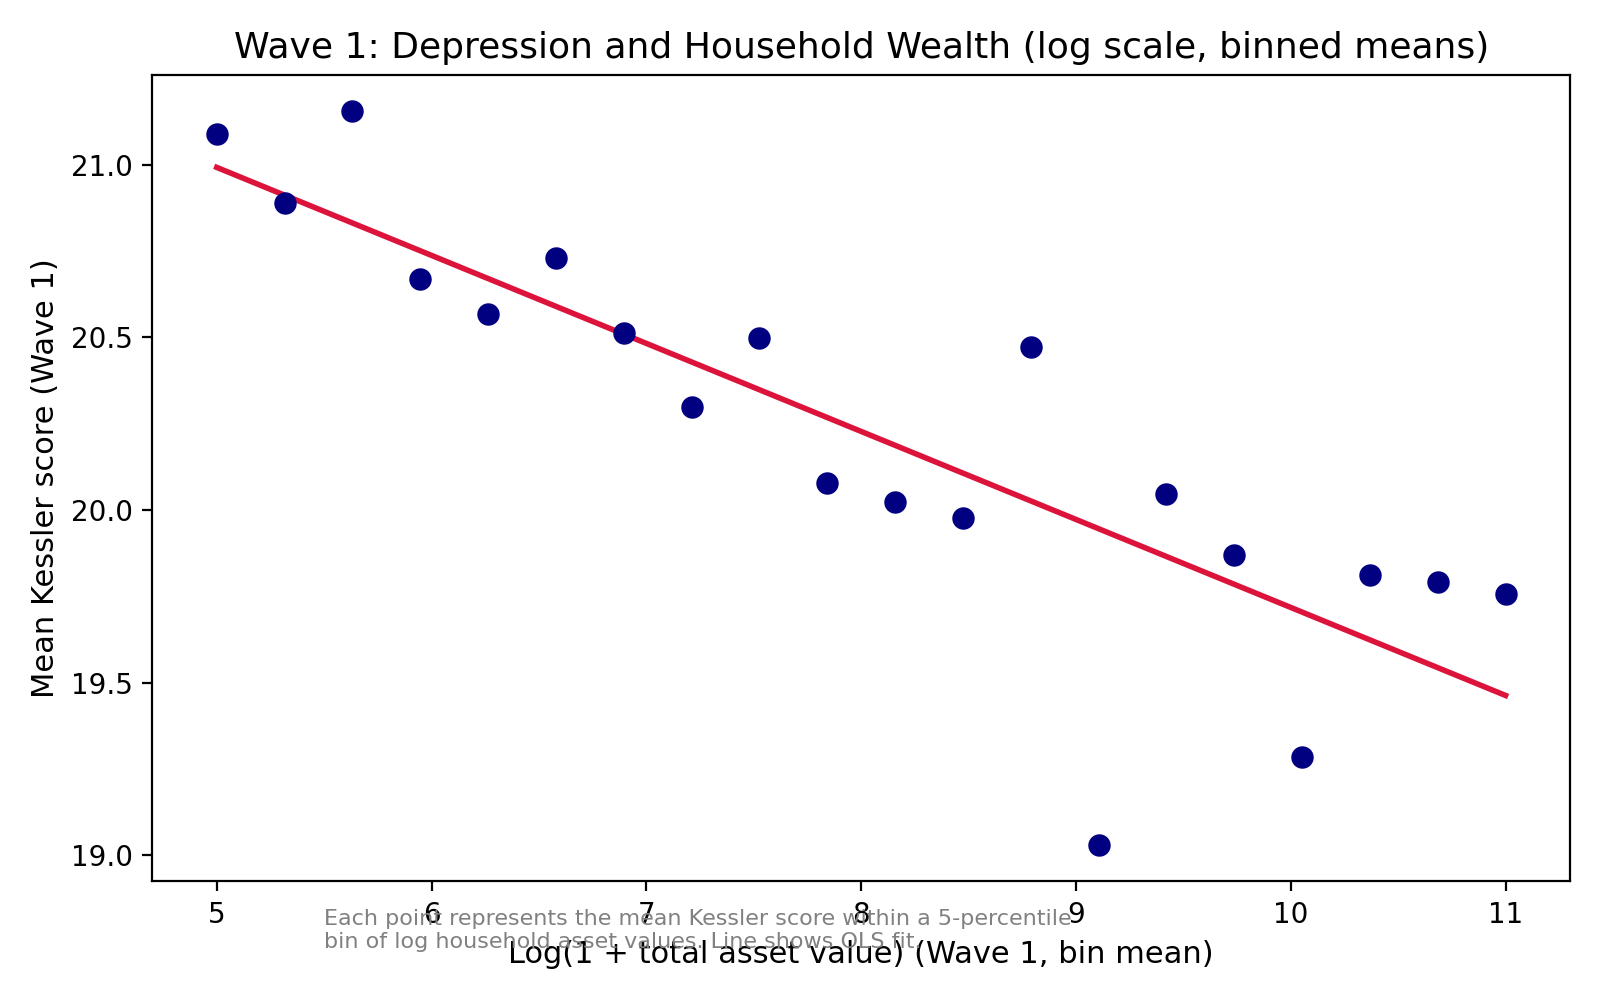
\includegraphics[width=0.85\textwidth]{fig_wealth_depression.png}
\caption{Wave 1: Depression and household wealth (binned means, log assets).}
\label{fig:wealth_depression}
\end{figure}

Figure~\ref{fig:wealth_depression} shows the relationship between household wealth and psychological distress at baseline, using binned averages of Kessler scores across the distribution of log household asset values. Each point represents the average Kessler score within a 5-percentile bin of the asset distribution, and the fitted line summarizes the overall trend.

The figure shows a negative relationship between household wealth and depression: individuals living in wealthier households tend to report slightly lower levels of psychological distress. While the relationship is not steep, the pattern is consistent across most of the asset distribution and suggests that economic conditions are correlated with baseline mental health outcomes.

\begin{table}[H]
\centering
\caption{Wave 1: Depression by Household Wealth Quartile}
\label{tab:wealth_quartile}
\begin{tabular}{lcccc}
\toprule
Wealth quartile & Observations & Mean Kessler score & Std.\ dev.\ & Severe depression (\%) \\
\midrule
Q1 (Poorest) & 1782 & 21.06 & 6.33 & 11.17 \\
Q2           & 1782 & 20.21 & 6.26 &  8.70 \\
Q3           & 1782 & 19.69 & 6.31 &  8.31 \\
Q4 (Richest) & 1781 & 20.18 & 6.25 &  8.48 \\
\bottomrule
\end{tabular}
\end{table}

Table~\ref{tab:wealth_quartile} presents baseline depression outcomes by household wealth quartile. Individuals in the poorest quartile report the highest levels of psychological distress, with an average Kessler score of 21.06, while individuals in the middle wealth quartiles exhibit somewhat lower mean scores. The prevalence of severe depression also declines across the wealth distribution, falling from 11.17\% in the poorest quartile to approximately 8--9\% in the upper quartiles. The differences across wealth groups are moderate in magnitude but broadly consistent with the negative association observed in Figure~\ref{fig:wealth_depression}.

\paragraph{Regression evidence.} To summarize the relationship between household wealth and psychological distress, I estimate a simple descriptive regression of the Kessler score on log household asset value using Wave~1 data:
\begin{equation}
\text{Kessler}_{ih} = \alpha + \beta \, \ln(\text{Assets}_h + 1) + \varepsilon_{ih},
\label{eq:wealth_reg}
\end{equation}
where $\text{Kessler}_{ih}$ denotes the depression score for individual $i$ in household $h$. Standard errors are clustered at the household level to account for within-household correlation in mental health outcomes.

\begin{table}[H]
\centering
\caption{Wave 1: Descriptive Regression of Depression on Household Wealth}
\label{tab:wealth_reg}
\begin{tabular}{lcc}
\toprule
 & (1) Bivariate & (2) With controls \\
\midrule
Log total asset value & $-0.215^{**}$ & $-0.191^{**}$ \\
 & (0.072) & (0.071) \\[4pt]
Age & & $0.008$ \\
 & & (0.005) \\[4pt]
Female & & $0.983^{***}$ \\
 & & (0.150) \\[4pt]
Household size & & $0.196^{***}$ \\
 & & (0.038) \\[4pt]
Constant & $21.981^{***}$ & $20.382^{***}$ \\
 & (0.569) & (0.622) \\
\midrule
Observations & 7127 & 7127 \\
\bottomrule
\end{tabular}
\begin{flushleft}
\small\textit{Notes:} Standard errors clustered at the household level in parentheses. $^{***}$ $p<0.01$, $^{**}$ $p<0.05$.
\end{flushleft}
\end{table}

The estimated coefficient on log household asset value is $-0.215$ (standard error 0.072), indicating that a one log-point increase in household assets is associated with a reduction of approximately 0.22 points in the Kessler depression score. Given that the average Kessler score in the sample is close to 20, this represents a modest but statistically significant association. Adding controls for age, gender, and household size attenuates the coefficient slightly to $-0.191$, confirming that the wealth-depression relationship is not driven by compositional differences across households.


\subsubsection{Depression and Gender}

Gender is a central dimension of heterogeneity in low-income settings because economic opportunities, control over resources, and exposure to risk often differ systematically for men and women. These differences can shape baseline well-being and the returns to household-level interventions. Classic evidence from rural Africa shows that gendered control over productive resources and intrahousehold allocation can be substantial, with implications for welfare and productivity \citep{Udry1996}. More broadly, development economists emphasize that gender-specific constraints and bargaining dynamics matter for policy design and targeting \citep{Duflo2012}.

\begin{table}[H]
\centering
\caption{Wave 1: Depression by Gender}
\label{tab:gender}
\begin{tabular}{lccc}
\toprule
Gender & Observations & Mean Kessler & Moderate/Severe (\%) \\
\midrule
Male   & 3162 & 19.70 & 20.43 \\
Female & 3965 & 20.75 & 26.48 \\
\bottomrule
\end{tabular}
\end{table}

Table~\ref{tab:gender} summarizes baseline depression outcomes by gender. Women report higher levels of psychological distress than men across multiple measures. The mean Kessler score for women is 20.75, compared to 19.70 for men. Similarly, 26.5\% of women fall into the moderate or severe depression range (Kessler score $\geq 25$), compared to 20.4\% of men.

\begin{figure}[H]
\centering
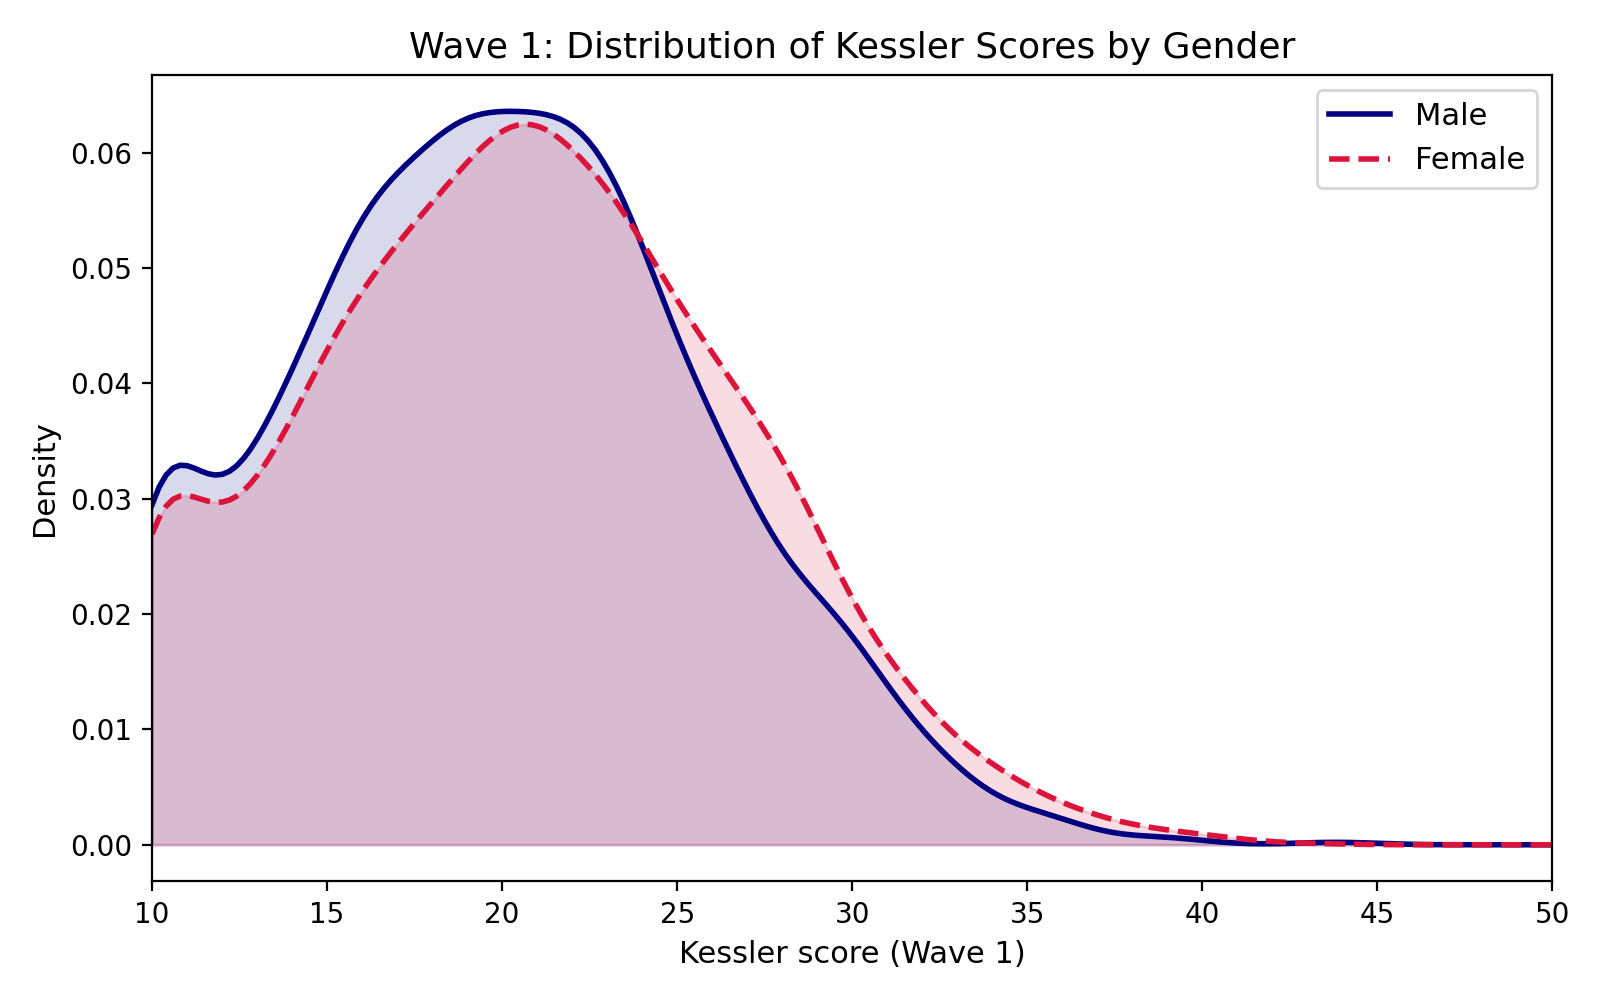
\includegraphics[width=0.85\textwidth]{fig_gender_density.png}
\caption{Wave 1: Distribution of Kessler scores by gender.}
\label{fig:gender_density}
\end{figure}

Figure~\ref{fig:gender_density} shows the distribution of Kessler depression scores by gender at baseline. The distributions for men and women are broadly similar in shape, with most individuals concentrated between Kessler scores of 15 and 25. However, the distribution for women appears slightly right-shifted relative to that for men, and women exhibit a somewhat heavier right tail, indicating a larger proportion experiencing high levels of psychological distress.

These results suggest that women experience a higher burden of psychological distress at baseline, consistent with evidence from low- and middle-income countries. The observed gender differences in baseline mental health motivate the later analysis examining whether the impact of Group Therapy differs by gender.


\subsubsection{Depression and Household Size}

Household size is economically relevant in environments with missing credit and insurance markets. Larger households can increase dependency burdens and resource strain, but may also provide informal risk-sharing and support. The net relationship between household size and well-being is therefore theoretically ambiguous and context-dependent \citep{Townsend1994}.

\begin{figure}[H]
\centering
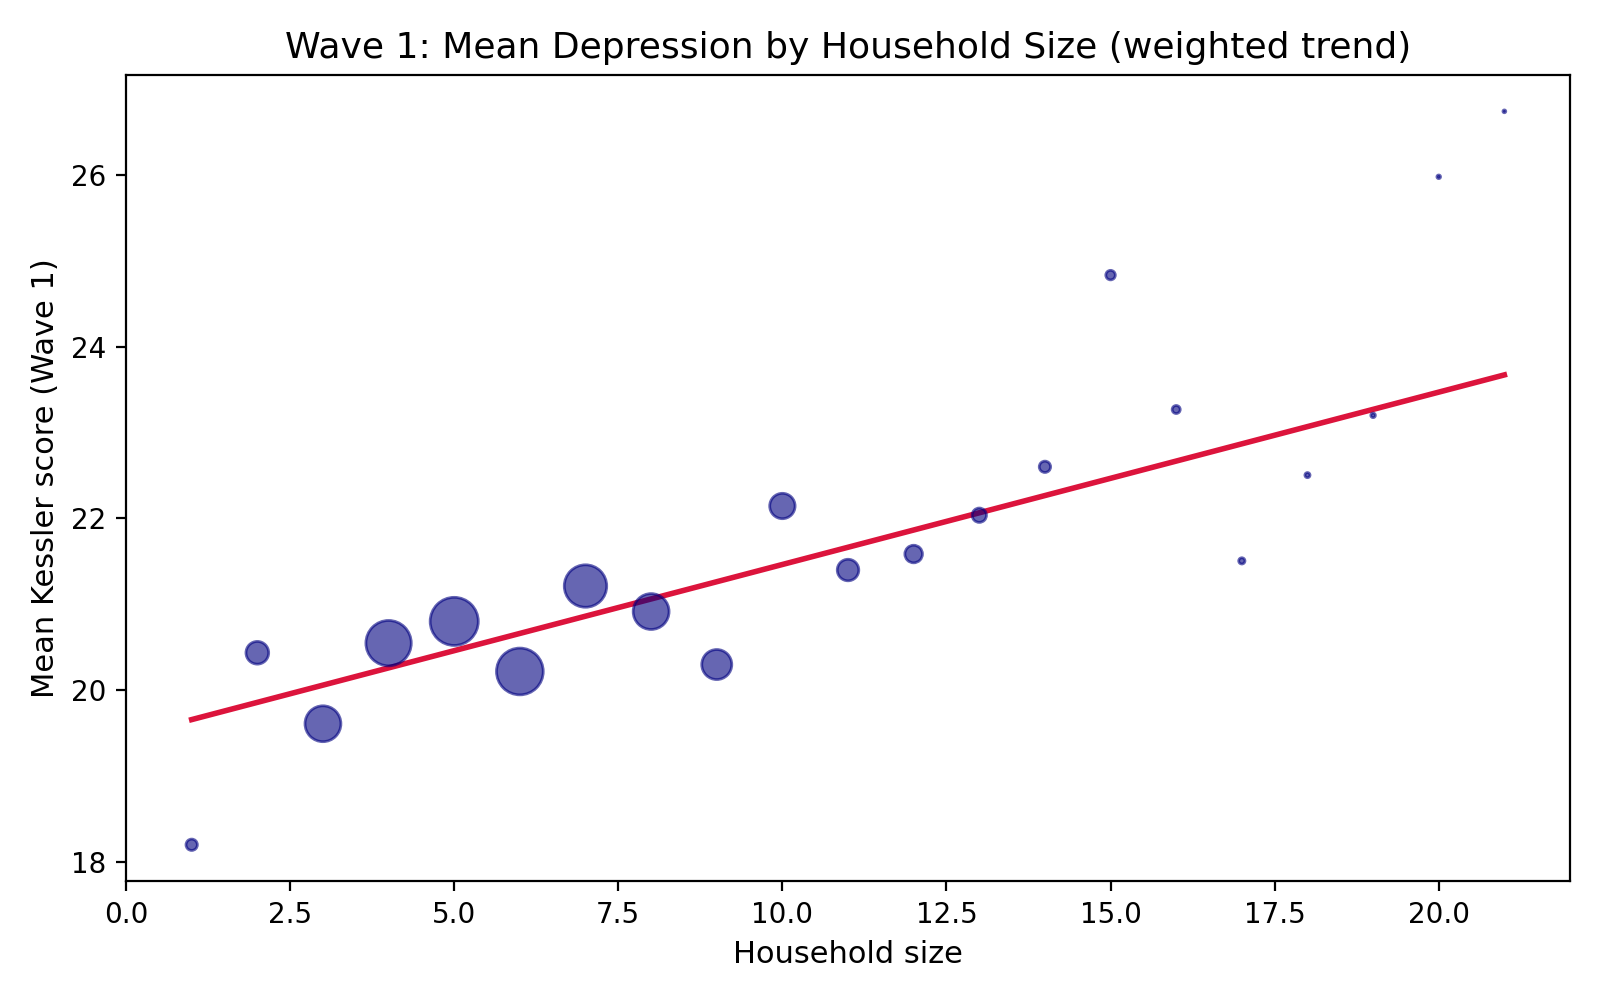
\includegraphics[width=0.85\textwidth]{fig_hhsize_depression.png}
\caption{Wave 1: Mean depression by household size group (with weighted trend).}
\label{fig:hhsize}
\end{figure}

Figure~\ref{fig:hhsize} shows the relationship between household size and psychological distress at baseline. For small and medium-sized households (approximately 1 to 8 members), average Kessler scores are relatively stable, with mean scores close to 20. For larger households, the average Kessler score appears to increase somewhat, though the pattern is irregular and likely reflects smaller sample sizes in the upper tail of the household-size distribution.

I estimate a simple descriptive regression:
\begin{equation}
\text{Kessler}_{ih} = \alpha + \beta \, \text{HHSize}_h + \varepsilon_{ih},
\end{equation}
with standard errors clustered at the household level.

\begin{table}[H]
\centering
\caption{Wave 1: Descriptive Regression of Depression on Household Size}
\label{tab:hhsize_reg}
\begin{tabular}{lc}
\toprule
 & (1) \\
\midrule
Household size & $0.226^{***}$ \\
 & (0.036) \\[4pt]
Constant & $19.319^{***}$ \\
 & (0.166) \\
\midrule
Observations & 7127 \\
\bottomrule
\end{tabular}
\begin{flushleft}
\small\textit{Notes:} Standard errors clustered at the household level. $^{***}$ $p<0.01$.
\end{flushleft}
\end{table}

The estimated coefficient on household size is 0.226, indicating that each additional household member is associated with an increase of approximately 0.23 points in the Kessler score. The positive coefficient suggests that individuals living in larger households tend to report slightly higher levels of psychological distress, possibly reflecting greater resource constraints. However, the magnitude is small relative to overall variation in depression scores, and the relationship between household size and depression appears modest compared to that between depression and household wealth or gender.


\section{Evaluating the RCT (Wave 2 Outcomes)}

\subsection{Were the GT Sessions Effective at Reducing Depression?}

Treatment effects are estimated using two specifications. The first is a simple difference-in-means estimator:
\begin{equation}
\text{Kessler}_{i2} = \alpha + \beta \, \text{Treat}_h + \varepsilon_{ih},
\end{equation}
where $\text{Kessler}_{i2}$ is the Wave~2 Kessler score for individual $i$ in household $h$, and $\text{Treat}_h$ is an indicator for treatment assignment.

The second specification uses an analysis-of-covariance (ANCOVA) model that controls for baseline mental health:
\begin{equation}
\text{Kessler}_{i2} = \alpha + \beta \, \text{Treat}_h + \gamma \, \text{Kessler}_{i1} + \varepsilon_{ih},
\end{equation}
where $\text{Kessler}_{i1}$ is the individual's baseline Kessler score. Standard errors are clustered at the household level in all specifications.

\begin{table}[H]
\centering
\caption{Treatment Effects on Depression (Wave 2 Outcomes), Clustered Standard Errors}
\label{tab:treatment}
\begin{tabular}{lccc}
\toprule
 & (1) Diff-in-means & (2) ANCOVA & (3) ANCOVA + controls \\
\midrule
Treated household & $-0.539^{***}$ & $-0.424^{**}$ & $-0.429^{**}$ \\
 & (0.157) & (0.162) & (0.162) \\[4pt]
Baseline Kessler (Wave 1) & & $0.157^{***}$ & $0.152^{***}$ \\
 & & (0.013) & (0.014) \\[4pt]
Constant & $17.521^{***}$ & $14.332^{***}$ & $14.185^{***}$ \\
 & (0.114) & (0.284) & (0.356) \\
\midrule
Observations & 6238 & 6238 & 6238 \\
\bottomrule
\end{tabular}
\begin{flushleft}
\small\textit{Notes:} Standard errors clustered at the household level in parentheses. $^{***}$ $p<0.01$, $^{**}$ $p<0.05$. Column~(3) additionally controls for age, gender, and household size.
\end{flushleft}
\end{table}

The ANCOVA specification is preferred to the simple difference-in-means because it improves precision by controlling for baseline mental health. Since Kessler scores are strongly correlated across survey rounds, conditioning on baseline values reduces residual variation. Under random assignment, both specifications provide unbiased estimates of the average treatment effect. However, ANCOVA typically produces smaller standard errors and therefore more precise inference, as evident in Table~\ref{tab:treatment}, where the coefficient on baseline Kessler score is highly significant. Including baseline outcomes is standard practice in randomized evaluations with pre-treatment data \citep{McKenzie2012, BruhnMcKenzie2009}.

The difference-in-means specification indicates that individuals in treated households have Kessler scores approximately 0.54 points lower than those in control households, statistically significant at the 1\% level. The ANCOVA specification produces a slightly smaller estimate of 0.42 points but remains statistically significant at the 5\% level. Adding demographic controls in column~(3) does not materially change the point estimate, providing reassurance that the randomization produced balanced treatment and control groups. Taken together, the results indicate that the Group Therapy sessions produced a modest but statistically significant reduction in psychological distress.


\subsection{Gender Heterogeneity in Treatment Effects}

To examine whether treatment effects differ by gender, I estimate the following regression using Wave~2 data:
\begin{equation}
\text{Kessler}_{i2} = \alpha + \beta_1 \, \text{Woman}_i + \beta_2 \, \text{Treat}_h + \beta_3 \, (\text{Woman}_i \times \text{Treat}_h) + \varepsilon_{ih},
\end{equation}
where $\text{Woman}_i$ is an indicator equal to one for female respondents and $\text{Treat}_h$ is an indicator for Group Therapy assignment. Standard errors are clustered at the household level.

\begin{table}[H]
\centering
\caption{Gender Heterogeneity in Treatment Effects (Wave 2), Clustered Standard Errors}
\label{tab:gender_het}
\begin{tabular}{lcc}
\toprule
 & (1) Prescribed spec.\ & (2) With baseline control \\
\midrule
Woman & $0.813^{***}$ & $0.614^{***}$ \\
 & (0.168) & (0.166) \\[4pt]
Treated household & $-0.130$ & $-0.077$ \\
 & (0.206) & (0.207) \\[4pt]
Woman $\times$ Treated household & $-0.723^{**}$ & $-0.612^{**}$ \\
 & (0.235) & (0.233) \\[4pt]
Baseline Kessler (Wave 1) & & $0.155^{***}$ \\
 & & (0.013) \\[4pt]
Constant & $17.061^{***}$ & $13.856^{***}$ \\
 & (0.147) & (0.286) \\
\midrule
Observations & 6238 & 6238 \\
\bottomrule
\end{tabular}
\begin{flushleft}
\small\textit{Notes:} Standard errors clustered at the household level. $^{***}$ $p<0.01$, $^{**}$ $p<0.05$. Total treatment effect for women $= \beta_2 + \beta_3$, tested using \texttt{lincom}.
\end{flushleft}
\end{table}

Table~\ref{tab:gender_het} reports the results. The constant term implies that men in control households have an average Kessler score of approximately 17.06 in Wave~2. The coefficient on Woman is 0.81 and statistically significant, indicating that women in control households report higher levels of psychological distress than men by about 0.8 Kessler points.

The coefficient on Treated household represents the treatment effect for men and is small and statistically insignificant ($-0.13$), suggesting little impact of the intervention on male respondents. The interaction term is negative and statistically significant ($-0.72$), indicating that women experienced substantially larger reductions in depression than men. Combining the coefficients, the total estimated treatment effect for women is approximately $-0.13 + (-0.72) = -0.85$ Kessler points. I formally test this linear combination using \texttt{lincom} and confirm it is statistically significant at the 1\% level.

These results suggest that the Group Therapy intervention was substantially more effective for women than for men. This pattern is consistent with the baseline evidence showing higher levels of psychological distress among women and suggests that the intervention may be particularly beneficial for populations with higher initial mental health needs.


\subsection{Economic and Policy Interpretation of Treatment Effects}

The estimates indicate that Group Therapy sessions reduced psychological distress by approximately 0.4--0.5 Kessler points on average. Given that the Kessler-10 scale ranges from 10 to 50, this corresponds to roughly a 2--3\% reduction relative to the control-group mean. The estimates are statistically precise and robust across specifications, indicating a clear improvement in mental health outcomes among treated households.

Interpreting the magnitude requires caution. A reduction of approximately half a point is unlikely to shift large numbers of individuals across clinical thresholds unless many respondents lie close to category cutoffs. However, the heterogeneity analysis indicates substantially larger impacts for women, with estimated reductions of approximately 0.8--0.9 Kessler points. Given that women exhibit higher baseline levels of distress, these subgroup effects are economically more meaningful.

Because compliance with treatment assignment was effectively perfect, the estimated coefficients can be interpreted as Average Treatment Effects (ATEs) rather than Local Average Treatment Effects (LATEs). This simplifies policy interpretation and provides a direct benchmark for expected impacts under full implementation, although realized effects could be smaller if compliance were lower at scale.

From an economic perspective, the key question is whether the magnitude of the effect justifies the resources required for implementation. Group-based delivery is typically less expensive than individualized therapy and has been implemented successfully in several low-income settings. If delivery costs are sufficiently low, modest improvements in mental health could still represent a cost-effective policy. However, without information on program costs or downstream economic outcomes such as labor supply, productivity, or household welfare, it is not possible to conduct a full cost-effectiveness assessment.

A further limitation is the relatively short follow-up horizon. Outcomes are measured approximately six months after the intervention, and prior research suggests that short-run improvements in psychological well-being may attenuate over time. If improvements translate into sustained changes in behavior and household welfare, the long-run benefits could be substantially larger than the short-run effects observed here. Conversely, if impacts fade quickly, continued or repeated interventions may be necessary.

Taken together, the results suggest that Group Therapy is a promising but not yet definitive policy intervention. A reasonable policy approach would involve incremental expansion combined with continued evaluation---particularly targeted at women and other populations with elevated baseline distress---rather than immediate large-scale rollout. It would be valuable to collect additional follow-up data, document program costs, and explore targeting strategies to strengthen the case for large-scale adoption.


\newpage
\appendix

\section*{Appendix A: Implementation and Packages}

\begin{itemize}
  \item \textbf{Data import:} Stata native \texttt{.dta} format; \texttt{destring} for type conversion.
  \item \textbf{Data cleaning and reshaping:} Core Stata commands (\texttt{bysort}, \texttt{egen}, \texttt{collapse}, \texttt{reshape}, \texttt{merge}).
  \item \textbf{Visualization:} Stata's \texttt{twoway} graphics.
  \item \textbf{Tables:} \texttt{estout} / \texttt{esttab} for \LaTeX{} export.
  \item \textbf{Regression:} \texttt{reghdfe} for fixed-effects specifications; \texttt{vce(cluster)} for household-clustered standard errors.
  \item \textbf{Hypothesis testing:} \texttt{lincom} for linear combinations of coefficients.
\end{itemize}


\section*{Appendix B: Key Assumptions}

\begin{itemize}
  \item Household size is measured at baseline (Wave~1 roster count) and held fixed for Wave~2.
  \item Missing unit asset values are imputed using item-level medians; total asset values are computed as quantity times imputed unit value and aggregated to household-wave.
  \item K10 scores are constructed by summing the ten items; observations with any missing K10 items are coded missing for the total score.
  \item Treatment assignment is household-level; standard errors are clustered at the household level.
  \item The analysis assumes full compliance with treatment assignment as specified in the task prompt.
\end{itemize}


\section*{Appendix C: AI Resource Guide}

Artificial intelligence tools were used as a supplementary resource during the completion of this task, consistent with the principle that AI complements rather than substitutes for independent analytical work.

First, AI tools assisted with debugging and formatting issues in Stata, particularly in resolving package conflicts, table export formatting, and do-file structure. This helped ensure that the final code runs cleanly and that output can be reproduced reliably.

Second, AI tools helped identify relevant academic literature on mental health and economic conditions in low- and middle-income countries, particularly studies related to asset-based wealth measurement and psychological interventions. The literature identified was subsequently verified and incorporated independently.

Third, AI tools served as a technical reference to clarify implementation details for standard empirical methods, including clustered standard errors, ANCOVA specifications, and interaction regressions.

At all stages, analytical decisions, econometric specifications, and interpretations were developed independently.


\newpage
\begin{thebibliography}{99}

\bibitem[Bruhn and McKenzie(2009)]{BruhnMcKenzie2009}
Bruhn, Miriam, and David McKenzie. 2009. ``In Pursuit of Balance: Randomization in Practice in Development Field Experiments.'' \textit{American Economic Journal: Applied Economics} 1(4): 200--232.

\bibitem[Duflo(2012)]{Duflo2012}
Duflo, Esther. 2012. ``Women Empowerment and Economic Development.'' \textit{Journal of Economic Literature} 50(4): 1051--1079.

\bibitem[Filmer and Pritchett(2001)]{FilmerPritchett2001}
Filmer, Deon, and Lant Pritchett. 2001. ``Estimating Wealth Effects Without Expenditure Data or Tears: An Application to Educational Enrollments in States of India.'' \textit{Demography} 38(1): 115--132.

\bibitem[McKenzie(2012)]{McKenzie2012}
McKenzie, David. 2012. ``Beyond Baseline and Follow-up: The Case for More T in Experiments.'' \textit{Journal of Development Economics} 99(2): 210--221.

\bibitem[Sahn and Stifel(2003)]{SahnStifel2003}
Sahn, David E., and David C. Stifel. 2003. ``Exploring Alternative Measures of Welfare in the Absence of Expenditure Data.'' \textit{Review of Income and Wealth} 49(4): 463--489.

\bibitem[Townsend(1994)]{Townsend1994}
Townsend, Robert M. 1994. ``Risk and Insurance in Village India.'' \textit{Econometrica} 62(3): 539--591.

\bibitem[Udry(1996)]{Udry1996}
Udry, Christopher. 1996. ``Gender, Agricultural Production, and the Theory of the Household.'' \textit{Journal of Political Economy} 104(5): 1010--1046.

\end{thebibliography}

\end{document}
